%!TEX root = ../main.tex

\graphicspath{{./figures/introduction/}}

\chapter{FISH-based transcriptomics}
\label{ch:introduction}

\minitoc
\newpage

My PhD thesis is devoted to the computational analysis of \ac{FISH} images in order to study subcellular localization of \ac{RNA}.
In this introduction, I will start by briefly presenting the fundamentals on gene expression and the role of \ac{RNA} localization therein.
Then, I will present the experimental protocols that allows us to visualize and analyse \ac{RNA} molecules as well as the Machine Learning methods I used.
I will finish this introduction with an overview of my thesis objectives, a list of the contributions I made and a summary of this manuscript to guide the reader.

\section{Gene expression}
\label{sec:gene_expression}

Cells are the basic unit of all living organisms.
They display an astonishing diversity in virtually all relevant aspects, and even cells belonging to the same organism are very different in terms of appearance and specific function they fulfill.
Yet, all cells belonging to the same organism share the same code, i.e.\space the same set of instructions, stored in the \ac{DNA}.
The \ac{DNA} corresponds to a long sequence of nucleotides, where the information on the living system is stored in form of a sequence of a 4-letter alphabet.
Genes are chunks of these long sequences that contain the blueprint for functional molecules.
The diversity of cells in terms of appearance and function is implemented by the production of different sets of these functional molecules.
This process is called gene expression.

Gene expression is the process by which genetic information is transformed into functional products.
\ac{RNA} molecules, or transcripts, are essential for this process.
They are either the functional gene products themselves or they serve as an intermediate molecule prior to the production of other functional products, namely the proteins.
A change in gene expression gives cells enough flexibility to adapt and react to different external stimuli.
It also drives cells differentiation, allows them to run their basic functions, modulate their activities and therefore appears to be one of the most fundamental processes of life.
On the contrary, its deregulation can lead to various diseases.
This explains the interest of the scientific community to study and decode gene expression processes.

In the living world, cells can be divided in two categories: prokaryotic cells, which do not have a nucleus and typically form a unicellular organism, and eukaryotic cells, with a well-organized nucleus.
An eukaryote (a living organism with eukaryotic cells) is usually composed of cells with a higher level of compartmentalization through membrane-bound organelles.
The nucleus is the place where most of the \ac{DNA} is stored.
The rest of the organelles are located in the cytoplasm, such as the mitochondria, the lysosomes, or the Golgi apparatus (see Figure~\ref{fig:eukaryotic_cell}).

For an eukaryotic cell, the expression of a gene includes two main steps: the transcription of a \ac{DNA} sequence into a \ac{RNA} (in the nucleus) and the translation of a \ac{RNA} into a protein.
Between these two major steps, there is a phase of maturation for the transcript, before a potential export outside the nucleus and a transport somewhere in the cytoplasm.
A cell can regulate either the transcription or the translation step to control the production of its functional molecules and thereby the biological process to which the proteins or \ac{RNA} contribute.

\begin{figure}[]
    \centering
    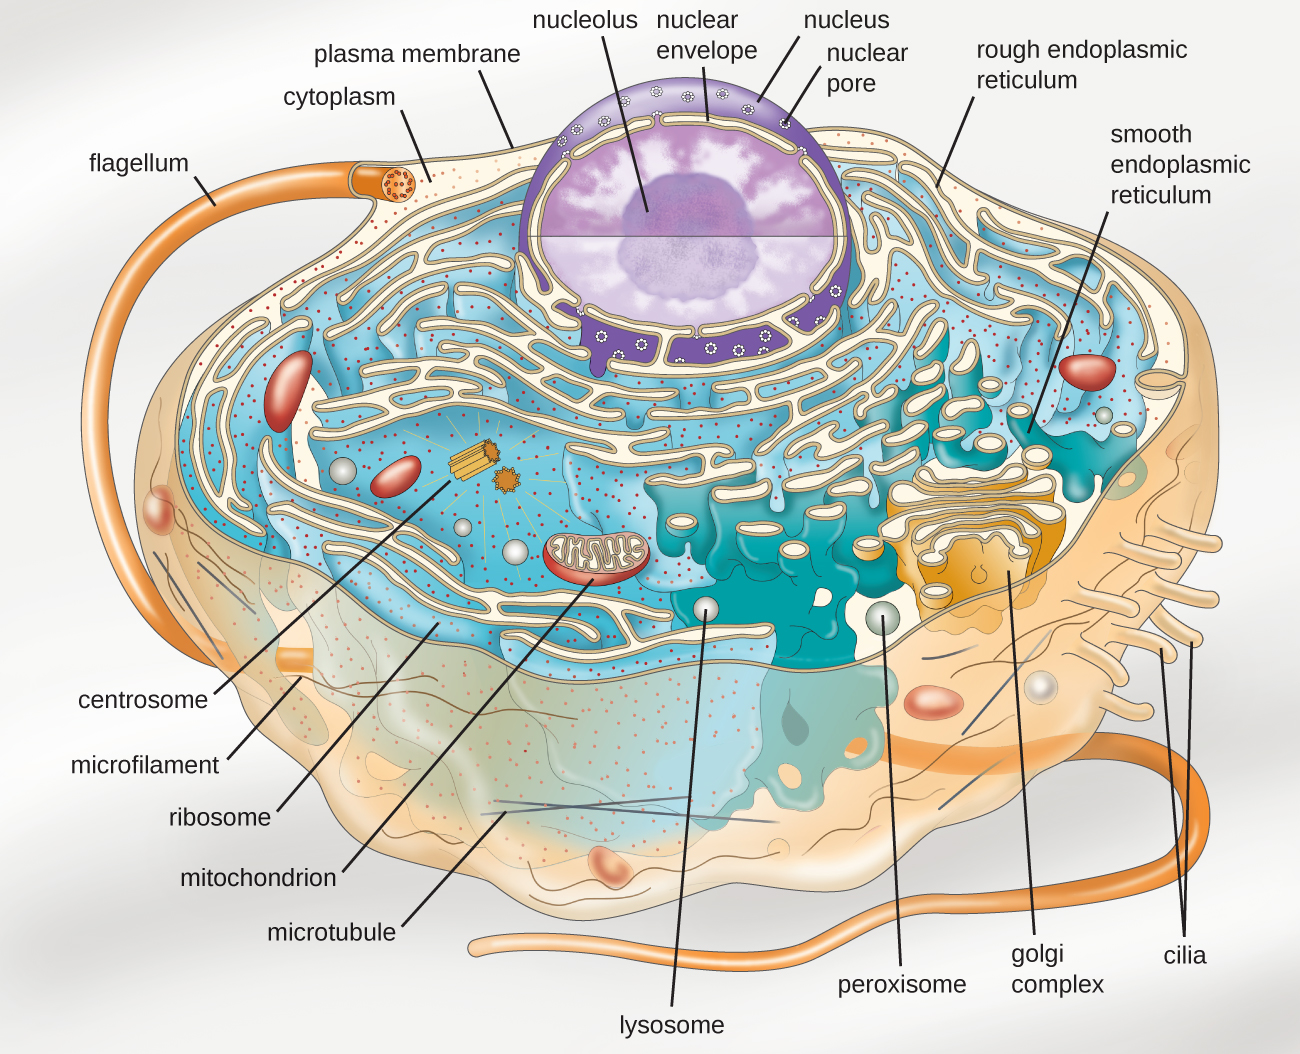
\includegraphics[width=0.8\textwidth]{figures/introduction/cell_eukaryotic.jpg}
    \caption[Illustration of an eukaryotic cell]{Illustration of an eukaryotic cell, from~\cite{parker2017microbiology}}
    \label{fig:eukaryotic_cell}
\end{figure}

\subsection{Transcription}
\label{subsec:intro_transcription}

\subsubsection{The primary transcripts}

This step consists in copying a gene (a sequence of nucleotides along the \ac{DNA} strands) into another biomolecule also composed of nucleotides: a \ac{RNA}.
While the \ac{DNA} is located within the nucleus, the \ac{RNA} can leave the nucleus by the nuclear pores.
\ac{RNA} can fulfill a number of different functions in the cell.
We distinguish two broad categories: \ac{mRNA} contain the blueprint for a protein that is synthesized outside the nucleus, while non-coding \ac{RNA} are not translated into a protein.
In a \ac{RNA}, the nucleotide Uracil (U) replaces the Thymine (T) and a ribose sugar serves as backbone instead of a desoxyribose sugar.
While both \ac{DNA} and \ac{RNA} contain genetic information, \ac{RNA} is a shorter single-stranded molecule, compared to the double-stranded \ac{DNA}, and is therefore less stable.
\ac{RNA} molecule also has two distinctive untranslated regions at its ends: 5'UTR and 3'UTR (corresponding to the number of carbon atoms in its sugar backbone extremities).\\

\noindent
Transcription proceeds as follows:
\begin{enumerate}
	\setlength\itemsep{0.1em}
	\item Proteins that serve as transcription factors bind to a specific sequence of \ac{DNA} (the promoter sequence) and recruit an enzyme (the \ac{RNA} polymerase) to initiate the transcription.
	\item The \ac{RNA} polymerase breaks the hydrogen bounds between the two \ac{DNA} strands to separate them.
	\item The \ac{RNA} polymerase moves along one \ac{DNA} strand, from 3' to 5' extremity, synthesizing a complementary nucleotides sequence on the way.
	\item The \ac{RNA} polymerase disengages from the strand when it meets a specific sequence of \ac{DNA} (the terminator sequence) and the newly synthesized nucleotides sequence (the primary transcribed \ac{RNA}) is released.
\end{enumerate}

\noindent
At this point, different sorts of \ac{RNA} are transcribed, depending of \ac{RNA} polymerase recruited:
\begin{itemize}
	\setlength\itemsep{0.1em}
	\item \ac{mRNA}, composed of coding (exon) and non-coding (intron) nucleotides, which conveys the blueprint of a future protein.
	\item \ac{rRNA} which, associated with ribosomal proteins, forms ribosomes, a macromolecular machine used by the cell to synthesize proteins.
	\item \ac{tRNA}, the most abundant \ac{RNA} molecule, which carries amino acids to the ribosome.
\end{itemize}

\begin{figure}[]
    \centering
    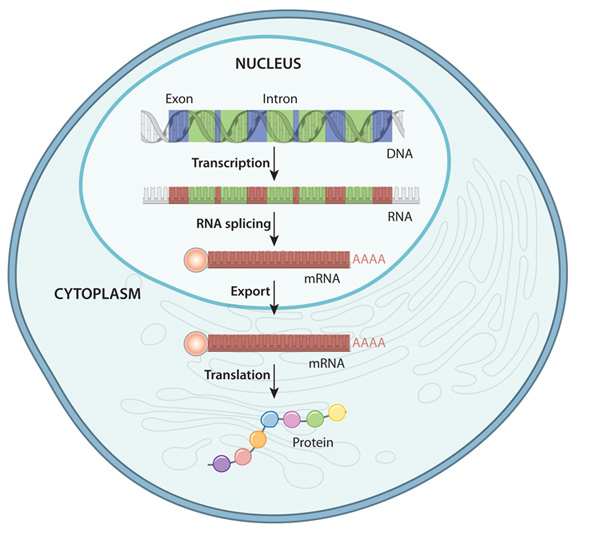
\includegraphics[width=0.8\textwidth]{figures/introduction/gene_expression_process.jpg}
    \caption[Schema of gene expression process]{Overview of gene expression process, from~\cite{cell_essential_nature}}
    \label{fig:gene_expression}
\end{figure}

\subsubsection{RNA maturation}

For the rest of the manuscript, I mainly focus on the \ac{mRNA}s.
They do not fit translation requirements yet and need to undergo three processes before leaving the nucleus:
\begin{itemize}
	\setlength\itemsep{0.1em}
	\item the 5' end is transformed (\ac{RNA} capping)
	\item a poly(A) tail (repeated adenine-based molecules) is added at the 3' end (polyadenylation)
	\item the non-coding parts of the \ac{RNA} sequence are removed (splicing)
\end{itemize}

\noindent
Those transformations enable to move the \ac{mRNA} out of the nucleus, regulate its degradation and promote the translation.
Figure~\ref{fig:gene_expression} shows a simplified illustration of the gene expression process.

\subsection{mRNA transport and localization}
\label{subsec:intro_rna_transport}

When an \ac{mRNA} is ready for export, it is moved out of the nucleus through the nuclear pore complex.
This complex recognizes a mature \ac{mRNA} if a specific set of proteins is bound to it - poly(a) binding proteins, cap binding proteins, and proteins related to the splicing step.
Once in the cytoplasm, an \ac{mRNA} is not necessarily exploited by a ribosome for translation.
It can also be silenced by translational repressors and stored, transported in a specific region of the cell or degraded.

Until recently, the scientific community thought translation mostly occurred at the endoplasmic reticulum and then proteins were transported where they were needed.
New evidence suggests on the contrary that \ac{mRNA} localization within the cell is not always random and \ac{mRNA}-protein colocalization could be an important aspect of cell organization and gene expression regulation~\cite{lecuyer_global_2007}.
However, the involved mechanisms are not well understood yet and the extend of \ac{mRNA}s concerned by a specific localization pattern is still unknown.
Beyond the number of \ac{mRNA} molecules within a cell (the expression level of a gene), researchers manifest now an increasing interest for \ac{mRNA} localization~\cite{Chin_lecuyer_2017}.

\subsubsection{mRNA transport}

There is a specific sequence in the 3'UTR of the \ac{mRNA} molecule that acts like a \emph{zipcode}~\cite{Chabanon_2004}.
This sequence can be recognized by a \ac{RBP} and starts the formation of a \ac{RNP} complex.
This structure is then central to coordinate the transport, the translation and the degradation of the \ac{mRNA} molecule throughout the cell.\\

\noindent
Three mechanisms to transport \ac{mRNA} or locally enrich them are identified (see Figure~\ref{fig:rna_transport} for illustration):
\begin{enumerate}
	\setlength\itemsep{0.1em}
	\item Active transport of \ac{mRNA}s along the cytoskeleton, potentially coupled with an anchoring mechanism.
	This is the most common transport mechanism observed.
	Motor proteins are recruited by the \ac{RBP}s, bind to the \ac{mRNA} complex and transport it along actin filaments or microtubules.
	\item At specific places, \ac{mRNA} molecules are protected from degradation complexes.
	This localization is then locally enriched and the spatial distribution of the transcript is biased in favor of these protected localizations.
	\item Transcripts diffuse randomly across the cell, but local entrapment make them accumulate with an asymmetric distribution.
	This mechanism is notably observed in bacteria, where no active transport of \ac{RNA} has been observed~\cite{das_intracellular_2021}.
\end{enumerate}

\begin{figure}[]
    \centering
    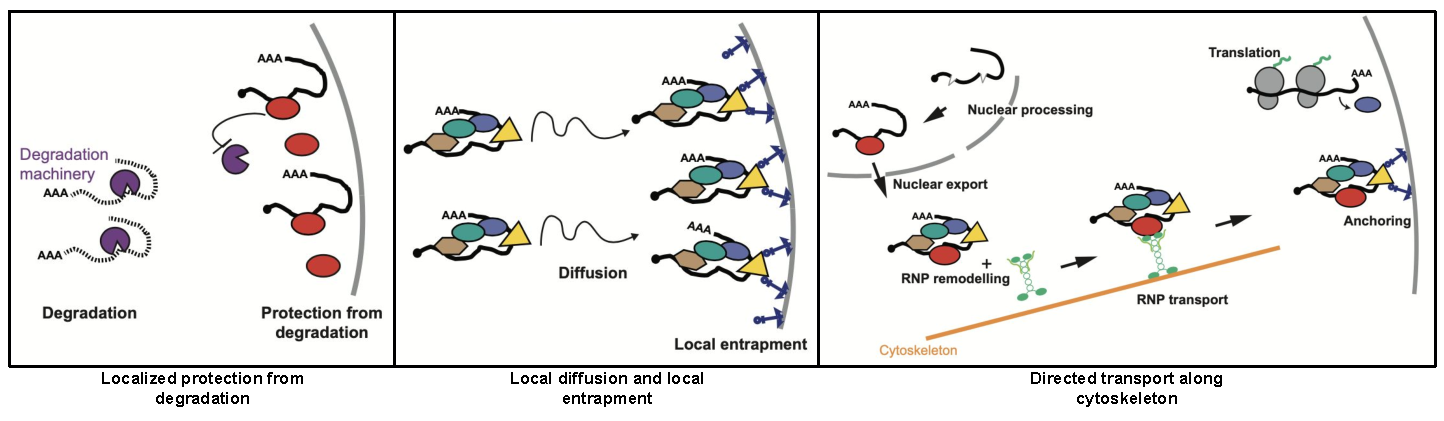
\includegraphics[width=\textwidth]{figures/introduction/rna_transport}
    \caption[Schema of RNA transport or locally enrichment mechanisms]{Schema of RNA transport or locally enrichment mechanisms, adapted from~\cite{Medioni_2012}.
	(\textit{Left}) RNAs are locally protected from degradation.
	(\textit{Center}) RNAs diffuse randomly, then they are locally entrapped.
	(\textit{Right}) RNAs are actively transported along cytoskeleton, thanks to RNP complexes and molecular motors.
	Directed transport can be coupled with an anchoring mechanism}
    \label{fig:rna_transport}
\end{figure}

\subsubsection{mRNA localization}

The localization of \ac{mRNA} can be see as an elegant and efficient mechanisms for the spatial regulation of gene expression.
By transporting one \ac{mRNA} molecule and promoting a local translation, several proteins can be directly produced at a desired place.
It saves the transport of a large amount of proteins~\cite{Medioni_2012}.
It also enables the cell to quickly react to external stimuli.
This mechanism could be critical to modulate the synaptic plasticity in neuron cells for example~\cite{jung_axonal_2012}.
Also, \ac{RNA} localization provides a mechanism to bring interaction partners in close proximity.
More generally, \ac{mRNA} localization will increase the cell compartmentalization and enable a higher flexibility and ''fine-tuning of gene expression in both space and time''~\cite{Medioni_2012}.

% mention Weeks et al. (1985) as first publication about RNA localization
% adham thesis: "Messenger localization was first discovered in Xenopus oocytes (Weeks et al., 1985)."

\subsection{Translation}
\label{subsec:intro_translation}

Finally, a cell synthesizes a protein through the translation process.
A ribosome is assembled around a \ac{mRNA} and moves along its nucleotides.
At the same time, \ac{tRNA}s carry amino acids matching the \ac{mRNA} sequence.
According to the genetic code, three successive nucleotides of the \ac{mRNA} (a codon) correspond to an amino acid.
The ribosome sequentially chains the amino acids, which then fold into a functional protein with a specific 3-dimensional structure.

\section{Imaging RNAs}
\label{sec:fish}

Traditional techniques to study gene expression are based on biochemical bulk-measurements, like microarrays~\cite{Schena_1995} or qRT-PCR~\cite{bustin_absolute_2000}.
They aim at identifying and quantifying the presence of \ac{RNA}s in a sample.
These methods could not operate at the single cell level and did therefore not allow to assess expression heterogeneity between cells.
Subsequent developments in next generation sequencing (NGS) allowed to address this limitation, by the advent of single cell \ac{RNA} sequencing~\cite{Hedlund_2018} or fluorescent in situ \ac{RNA} sequencing (FISSEQ)~\cite{Church_2014}.

An alternative option is to rely on images, which naturally provide insights regarding the spatial distribution of \ac{RNA}s and, with sufficient resolution, enable single cell analysis.
Coupled with techniques from High Content Screening --- a largely automatized experimental setup --- this approach can be applied at a large scale, probing thousands of \ac{RNA}s with respect to their spatial localization.

\begin{figure}[]
    \centering
    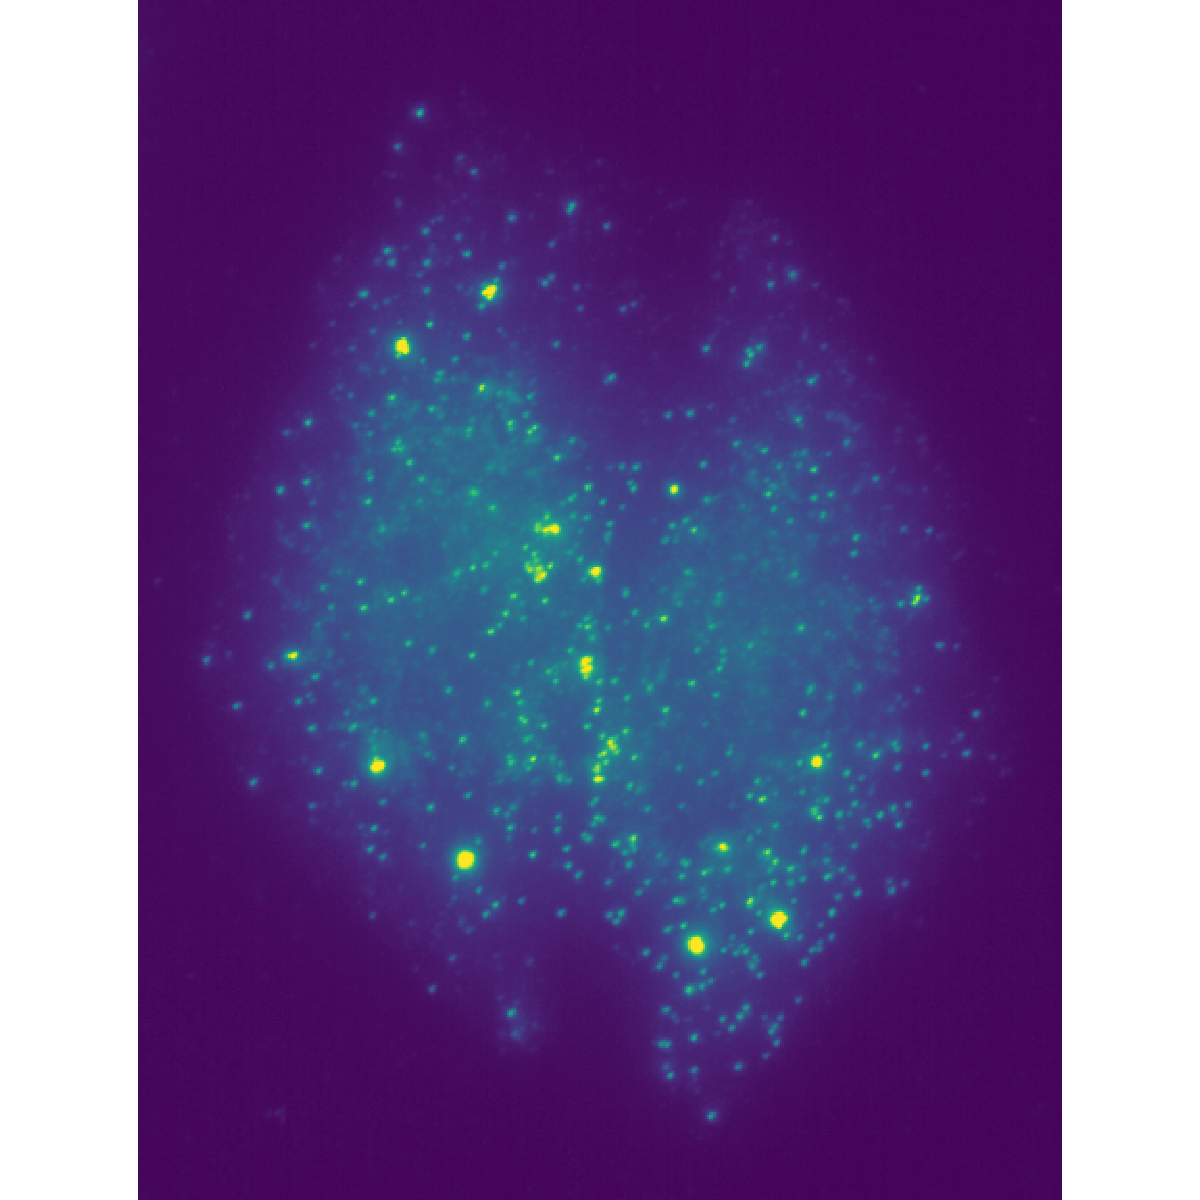
\includegraphics[width=0.7\textwidth]{figures/introduction/multichannel_input}
	\caption[Example of smiFISH image]{Example of smiFISH images with a maximum intensity projection.
	Each spot is a single RNA molecule}
    \label{fig:smFISH_input}
\end{figure}

\subsection{The smFISH experiment}
\label{subsec:intro_smfish}

Notably, \ac{smFISH} technique~\cite{Femino_1998}, is the first to reach single molecule resolution in fixed cells.
It uses multiple fluorescent oligonucleotides (or probes) that hybridize to the target RNA.
Importantly, this technique preserves the cell environment, and thus enriches the contextual information available in the images.
However, probes need to be specifically designed against the transcript of interest, making this solution costly to scale.
A \ac{smFISH} experiment includes four steps:

\begin{enumerate}
	\setlength\itemsep{0.1em}
	\item Cell fixation and permeabilization
	\item Hybridization of the fluorescent probes for several hours
	\item Cell washing to remove unbound probes
	\item Image acquisition under a wide field microscope
\end{enumerate}

\noindent
As \ac{RNA} molecules are smaller than the diffraction limit of the microscope, the final image results in diffraction limited spots over a fluorescent background (see Figure~\ref{fig:smFISH_input}).
In \ac{smFISH} images, we do not observe the actual molecule, but its \ac{PSF}.
The background comes from both the cellular autofluorescence and the unbound probes.
Single \ac{RNA} molecule can be resolved because of the hybridizations of multiple fluorescent probes on the same molecule.
This technique increases the \ac{SNR} and ensures that the \ac{RNA} signal is brighter than the background.

\begin{wrapfigure}{R}{0.50\textwidth}
	\begin{center}
	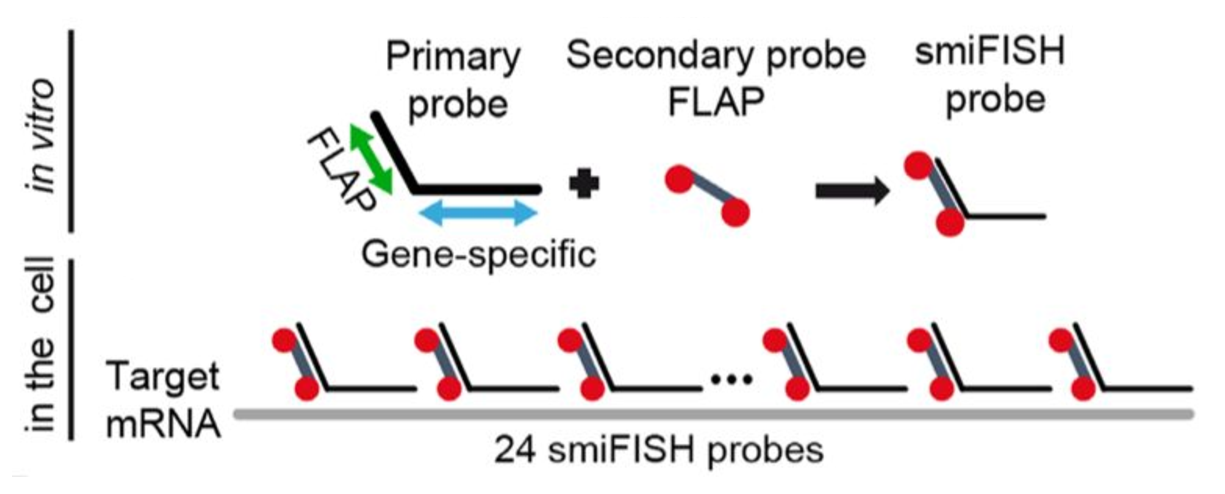
\includegraphics[width=\linewidth]{figures/introduction/smiFISH}
	\caption[Schema of smiFISH protocol]{Schema of smiFISH protocol from~\cite{tsanov_smifish_2016}}
	\label{fig:smiFISH}
	\end{center}
\end{wrapfigure}

In~\cite{tsanov_smifish_2016}, a cheaper and simpler version of \ac{smFISH} is presented: \ac{smiFISH}.
The fluorescent probe is built through a pre-hybridization step that matches a primary (unlabeled) probe with a secondary fluorescent oligonucleotide (see Figure~\ref{fig:smiFISH}).
This design with indirect labeling presents a higher flexibility and saves cost.

\subsection{Large-scale FISH studies}
\label{subsec:intro_scale_fish}

FISH is an experimental technique compatible with large-scale studies.
The first large scale screen focusing on RNA localization was performed in Drosophila embryos~\cite{lecuyer_global_2007} and revealed a surprising number of \ac{mRNA}s that have preferential localization during embryogenesis ($71\%$ out of more than 3000 genes tested). 

A large-scale screen in mammalian cell lines was proposed a few years later~\cite{battich_image-based_2013, battich_control_2015}, assessing the transcriptional noise and their relationship to cellular phenotypes, as well as subcellular localization of \ac{mRNA}s for a large number of genes ($N = 1000$).

Our collaborators also adapted our \ac{smiFISH} protocol to 96-well plates, permitting robotized experiments and automated imaging to study hundreds of \ac{RNA} species~\cite{tsanov_smifish_2016, safieddine_choreography_2021}.

One of the limitations of these \ac{smFISH} approaches with respect to single cell RNAseq is that they only visualize the localization and expression of transcripts one \ac{RNA} species at a time.
More recent developments relying on sequential hybridization steps and barcoding \ac{RNA}s, allow now the joint analysis of hundreds of \ac{RNA}s in the same cells~\cite{lubeck_single_cell_2014, Chen_2015, eng_seqfish_2019, fazalAtlasSubcellularRNA2019}.
These techniques were not available in practice at the time of the data collection for this PhD thesis, but in principle, they represent a very interesting alternative to High Content Screening.

\section{Measuring images: from pixels to numbers}
\label{sec:computation_biology}

\subsection{Working with bioimages}
\label{subsec:intro_bioimages}

Over the past decades, a number of technological breakthroughs and new experimental techniques have transformed biology in depth.
The availability of large, systematically acquired datasets allow today to perform integrated systems-level analyses.
This transformation also significantly increases the importance of data collection and maintenance, as well as robust quantitative approaches allowing to extract valuable insights from these datasets.

In bioimaging specifically, current experimental platforms allow us to perform a large number of experiments under varied conditions and highly informative content.
These techniques are referred as High Content Screening and pave the way for a systematic analysis of living systems.
Finally, the increasing degree of automation of experimental protocols justifies the development of bioimage informatics as a discipline in its own right to assist biologists.

The use of images in biology brings several advantages: (1) images are informative about morphological phenotypes, (2) they preserve the spatial dimension of the living system studied, as well as the temporal dimension in the case of repeated image acquisitions in live imaging experiments and (3) they allow to access different scales of organization, from the molecular scale to the tissue architecture.

Bioimage Informatics deals with all computational aspects of images in the life sciences.
There is a large variety of different tasks, such as image restoration, denoising, segmentation, tracking, registration and recognition of specific phenotypes.
Usually, image datasets are characterized by an important variability: living systems can be imaged at different scales, with different modalities of acquisition and evolving technology.
In addition, the fluorescent markers used in microscopy or the question investigated by researcher may differ, making images of the same object from two different studies not necessarily compatible.
As a consequence, the field often requires tailored solutions to the problem at hand.
However, there can also be for some projects a common algorithmic backbone, that just needs to be adapted to new projects.

\subsection{Machine Learning for bioimages}
\label{subsec:intro_ml_tools}

\subsubsection{A Machine Learning boom}

The recent years have seen a renewed interest for Machine Learning research, the cornerstone of current artificial intelligence era, driven by successful applications in vision, language understanding, speech recognition, etc\dots
This term of Machine Learning was coined to describe the set of techniques and models that make automatic decision based on patterns \emph{learned} and found in data.
For some specific tasks (like image classification) these algorithms have reached human-like capabilities.
For other fields, the gap between computer and human performances keeps decreasing.
In computer vision, the success of Machine Learning models makes their use legitimate for bioimage informatics applications.\\

\noindent
Overall, three ingredients make these successes possible:
\begin{enumerate}
	\setlength\itemsep{0.1em}
	\item methodological advances regarding the predictive models
	\item large annotated datasets
	\item increased computing power to process an ever growing number of operations
\end{enumerate}

\noindent
While new developments certainly are important for the performance of Machine Learning, it must be noted that many of the principles in Machine Learning and Deep Learning in particular (a family of Machine Learning models based on artificial neural networks) have been studied and developed for decades (see~\cite{Bishop_2006, hastie_elements_2009} for a review of different Machine Learning methods).
Convolutional Neural Networks, which are the most widely used neural networks in Computer Vision, were developed more than 25 years ago~\cite{LeCun1998}, but became the state-of-the-art method only after 2012~\cite{alexnet_2012}, when they won a classification challenge on a large dataset of natural images~\cite{Deng_2009}.
In biomedical community, Machine Learning techniques are disseminating and address more challenges every year (see~\cite{jumper_highly_2021} for an example with the protein folding problem).

\subsubsection{Neural networks as the next generation tool}

In case of Deep Learning, model architectures are based on neural networks with successive layers of artificial neurons.
Each neuron is defined by a set of weights and perform a linear combination of the input signal with its weights, followed by a potential non linear transformation (usually a \emph{maxout}, \emph{sigmoid} or \emph{tanh} function).
A complete network usually combines these layers of neurons with normalization steps.
It can be seen as a parametrized model, whose weights need to be optimized to minimize for a specific task.

Given an input, a loss function enables to compare the output signal of the model with a ground truth (the expected output signal) and thus compute a gradient (the first order derivative of the loss function).
The backpropagation of this gradient to the rest of the network makes it possible to update the weights of the layers in order to minimize the loss~\cite{rumelhart_learning_1986}.
This process defines a training step.
After several iterations, the loss and the gradient should decrease, and the network progressively stabilizes its weights.
The weights are ultimately frozen and the model is trained.

Such architecture is highly flexible and different variants have been developed~\cite{lecun_deep_2015}.
For a general introduction to Deep Learning techniques, one can refer to~\cite{Goodfellow_2016}.

\subsubsection{Limitations and caveats}

Beyond the great performances returned by Machine Learning models, a number of limitations and caveats should be considered.

First, they require annotated datasets to train and evaluate the models.
Compared to natural images, this ground truth is particularly costly to obtained with biomedical images as it often involves the assignation of experts (medical doctor or biologists) to a time-consuming, repetitive and annoying task.
As a consequence, datasets available for a given biomedical problem are often too small, highly diversified or released without any useful manual annotations.

Second, Machine Learning algorithms require robust evaluation protocols, strong benchmarks and a rigorous choice of evaluation metrics\footnote{One can see~\cite{varoquaux_machine_2022} for a description of these evaluation caveats when Machine Learning models are applied to medical images.}.
It is necessary to prevent data leakage and firmly separate the training set from the test set in our dataset, otherwise models overfit to the training samples and generalize poorly to unknown data.
If the test set is not representative of the data distribution, or too small, the evaluation will be biased and hardly reproducible~\cite{Varoquaux_cv_2018}.
Obviously, all these limitations are worsened by the inherent heterogeneity of bioimages and the difficulty to assemble manual annotations.
Working with Machine Learning models, one needs strong and diversified baselines that reflect the state-of-the-art of performances, as well as the right choice of metrics to benchmark the developed methods with respect to approaches published in the literature.

Third, flexibility of some models comes at a price: a sensitivity to the selected hyperparameters, which makes the evaluation all the more important.

Last but not least, most of the Deep Learning models appear like a black box solution with an internal process that cannot be easily or directly interpreted.
While this problem is more critical for direct medical applications than biological ones, it requires an important pedagogical effort to diffuse Deep Learning techniques to the rest of the scientific community.

\section{Goals and contributions}
\label{sec:contributions}

\subsection{Goals}
\label{subsec:intro_goals}

\begin{figure}[]
	\centering
	\minipage{0.2\textwidth}
		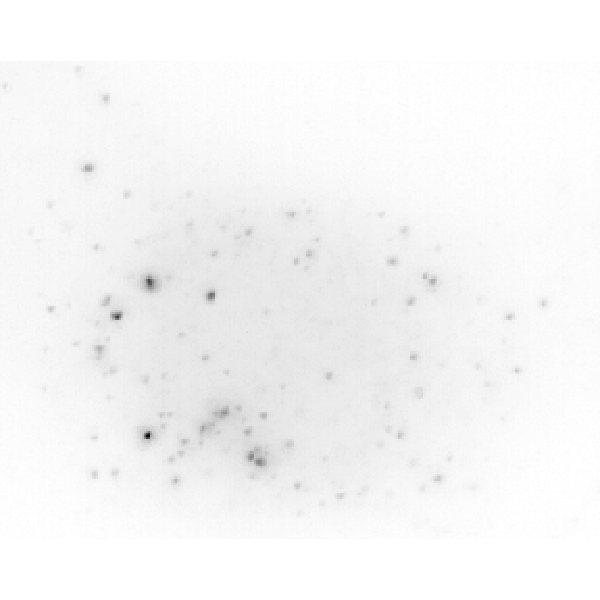
\includegraphics[width=0.95\linewidth]{figures/introduction/real_image_foci}
		\vfill
		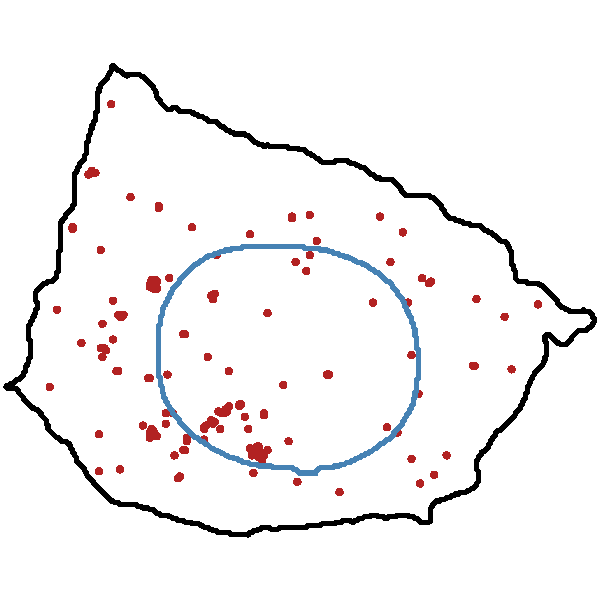
\includegraphics[width=0.95\linewidth]{figures/introduction/real_coord_foci}
		\subcaption{Foci}
	\endminipage\hfill
	\minipage{0.2\textwidth}
		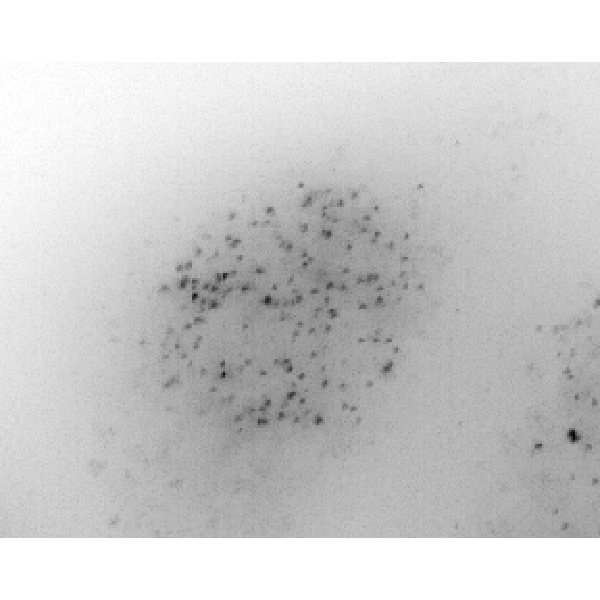
\includegraphics[width=0.95\linewidth]{figures/introduction/real_image_intranuclear}
		\vfill
		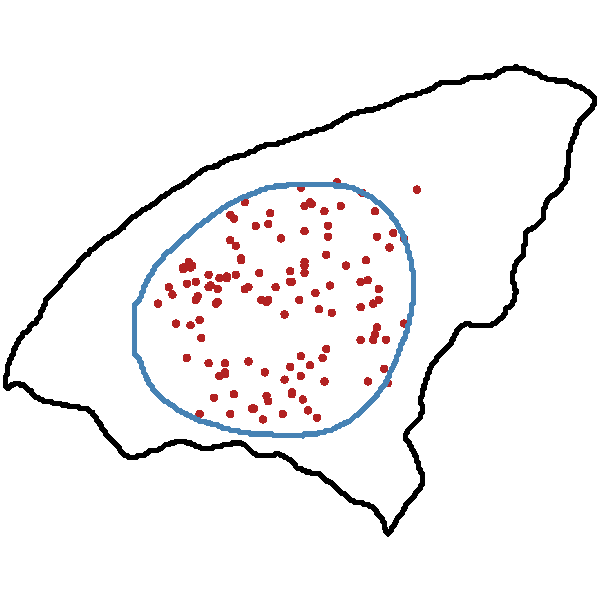
\includegraphics[width=0.95\linewidth]{figures/introduction/real_coord_intranuclear}
		\subcaption{Intranuclear}
	\endminipage\hfill
	\minipage{0.2\textwidth}
		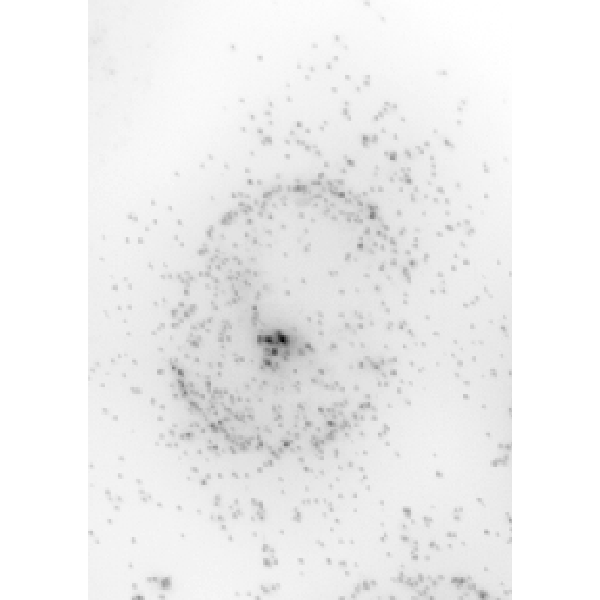
\includegraphics[width=0.95\linewidth]{figures/introduction/real_image_nuclear_edge}
		\vfill
		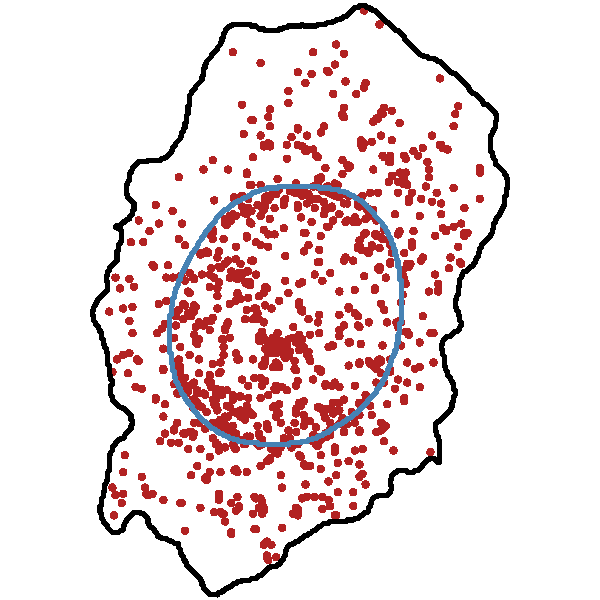
\includegraphics[width=0.95\linewidth]{figures/introduction/real_coord_nuclear_edge}
		\subcaption{Nuclear edge}
	\endminipage\hfill
	\minipage{0.2\textwidth}
		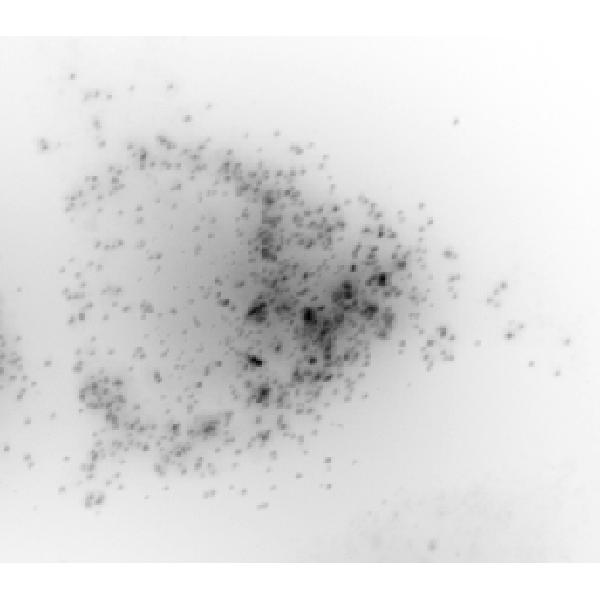
\includegraphics[width=0.95\linewidth]{figures/introduction/real_image_perinuclear}
		\vfill
		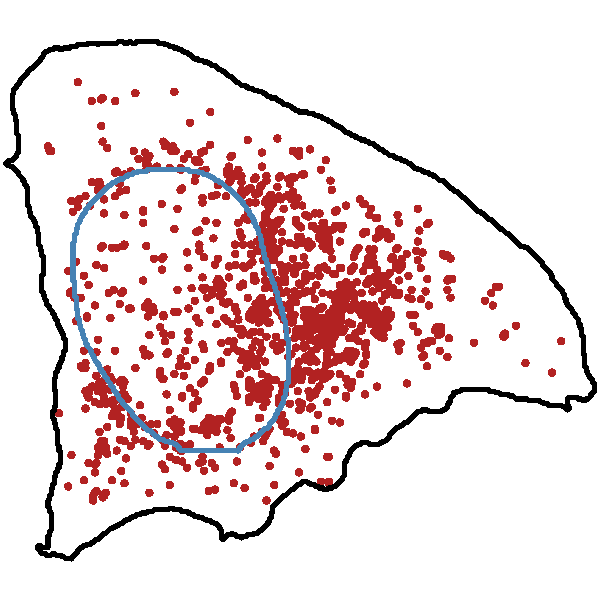
\includegraphics[width=0.95\linewidth]{figures/introduction/real_coord_perinuclear}
		\subcaption{Perinuclear}
	\endminipage\hfill
	\minipage{0.2\textwidth}
		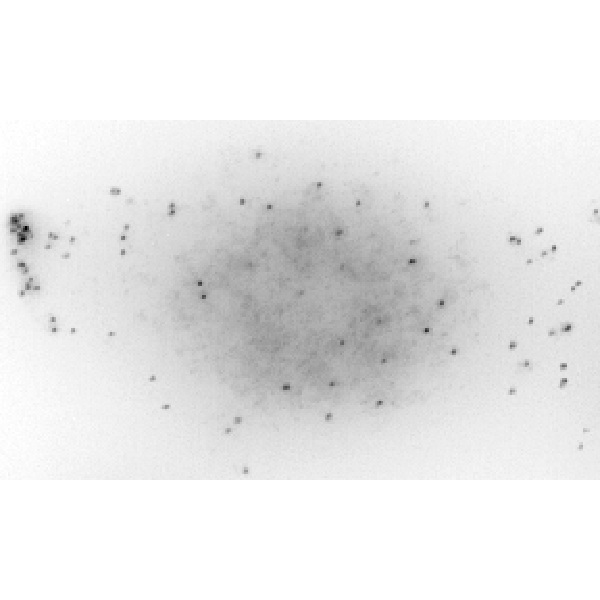
\includegraphics[width=0.95\linewidth]{figures/introduction/real_image_protrusion}
		\vfill
		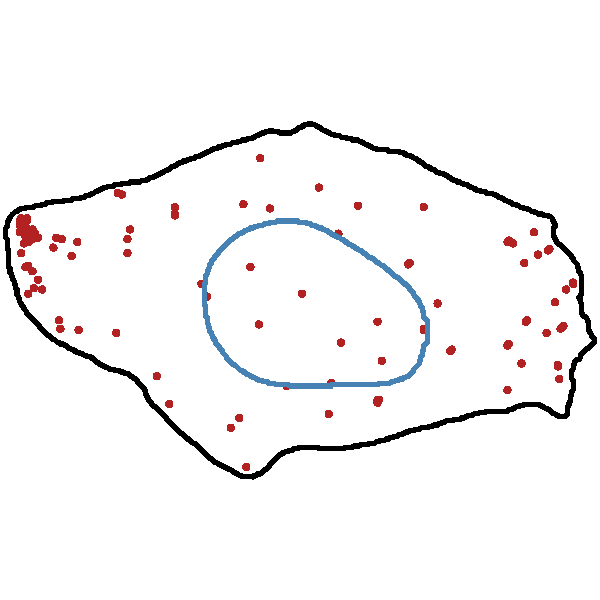
\includegraphics[width=0.95\linewidth]{figures/introduction/real_coord_protrusion}
		\subcaption{Protrusion}
	\endminipage
	\caption[RNA localization patterns from pixels to numbers]{RNA localization patterns from~\cite{pointfish_2022}.
	(\textit{Top}) Typical smFISH images with different RNA localization patterns.
	(\textit{Bottom}) Coordinate representations with RNA spots (\textit{red}), cell membrane (\textit{black}) and nuclear membrane (\textit{blue}).
	Detection and segmentation results are extracted and visualized with FISH-quant~\cite{Imbert_fq_2022}}
	\label{fig:intro_localization_patterns}
\end{figure}

My PhD had three main objectives:

\begin{enumerate}
	\setlength\itemsep{0.1em}
	\item Development of a full workflow for the analysis of \ac{smFISH} images, containing state-of-the-art methods for image segmentation (nucleus and cytoplasm), a robust method for \ac{RNA} detection applicable to large-scale screens and classification of \ac{RNA} localization patterns.
	\item Implementation of the methods in a python based open source tool, usable by the scientific community.
	\item Application of the developed methods and tools to real experimental datasets in ongoing screens on subcellular \ac{RNA} localization.
\end{enumerate}

Figure~\ref{fig:intro_localization_patterns} illustrates the gap that needs to be bridged between the input images and an adequate representation of the \ac{RNA} localization, making their quantitative analysis possible.

\subsection{Contributions}
\label{subsec:intro_contributions}

Beyond this manuscript and the publications, my contributions are essentially lines of code.
In an effort of transparency, reproducibility and documentation, I developed computational tools as useful as possible for any biologist interested in \ac{FISH} experiments.
My PhD results in three major contributions.

\begin{itemize}
	\setlength\itemsep{0.1em}
	\item My first and main contribution is FISH-quant V2.
	This online framework gathers Python packages and a \ac{GUI} to process \ac{FISH} images, build robust analysis pipelines and perform simulations.
	\item My second contribution is an alternative method to compute relevant features in order to discriminate \ac{RNA} localization patterns.
	This method implied the development of PointFISH, a dedicated Deep Learning model operating directly on point clouds.
	\item My third contribution was the participation in biological studies, where I could apply the computational methods and tools I had developed.
	These studies leveraged high content screening assays and \ac{smFISH} techniques to perform a systemic analysis of \ac{RNA} localization and investigate local translation.
\end{itemize}

\noindent
Additional contributions are mentioned throughout this manuscript, including the annotation of a dataset for nucleus and cell segmentation with thousands of instances and the supervision of an intern.
The work performed during this internship was the seed for the first publication of another PhD student in the team, about in silico labeling and segmentation.
Lastly, a list of my publications are available at the very end of the manuscript.

\subsection{Manuscript summary}
\label{subsec:intro_manuscript}

The manuscript is composed of two parts.
The first four chapters are a presentation of the analysis pipeline with a focus on every critical stage.
It includes systematic reviews of the existing methods and details about solutions I implemented.
In addition, code snippets, ready to be imported and run, are interspersed with descriptions of the related algorithms.
The second part details several applications of my tools, where quantification of \ac{RNA} localization patterns provides biological insights.

In \textbf{Chapter~\ref{ch:chapter1}}, I give an overview over the general computational framework and the design of the software I have developed and published during my PhD thesis: FISH-quant v2.
It includes methods for every stage of a \ac{FISH}-based analysis, with an effort to make them scalable and modular.
I also describe the improvements from the original FISH-quant version in MATLAB, and how they address the requirements of a modern software tool.

In \textbf{Chapter~\ref{ch:chapter2}}, I focus on \ac{RNA} detection.
With \ac{smFISH} experiments, the \ac{RNA} molecules are spotted and reduced to discrete data points in space.
I describe detection algorithms and their extensions available in FISH-quant.
In the end, the set of all \ac{RNA} molecules is reduced to a point cloud with spatial coordinates.

In \textbf{Chapter~\ref{ch:chapter3}}, I review and describe algorithms for nucleus and cell segmentation.
Most of them are Deep Learning models, trained on vast datasets of annotated images.
Beside my own implemented methods, I also present refinement techniques to improve and format segmentation masks.
Two other projects for which I contributed (including one published) are also discussed at the end of the chapter.
They aim at improving the efficiency and consistency of segmentation on specific aspects.

In \textbf{Chapter~\ref{ch:chapter4}}, I compare two different approaches to quantify \ac{RNA} localization patterns.
Once the \ac{RNA} molecules are detected and cell morphology is segmented, the pixel domain gives way to Euclidean space and cells can be represented with a coordinate representation.
Then, spatial features are computed in order to discriminate relevant localization patterns.
I present two different methods of feature engineering.
The first method consists in manually designing features to characterize specific localization patterns.
I then list and describe every hand-crafted feature implemented in FISH-quant.
The second (published) method consists in learning features.
They are extracted from a Deep Learning model fed with the \ac{RNA} point cloud as input and trained on a simulated pretext task.

In \textbf{Chapter~\ref{ch:chapter5}}, I present several applications of my quantitative pipeline.
These applications come from three publications where we study different \ac{RNA} localization patterns.
I designed a classification pipeline to recognize a variety of localization patterns.
An additional series of experiments which I computationally analyzed, led to the discovery of translation factories, a novel mechanism for the spatial control of gene expression.
In a different screen, I developed additional features to quantify a cell cycle dependent pattern, which is related to centrosomes.
Finally, I also contributed to a study focused on the protrusion pattern, where \ac{RNA} localize in cell extensions.